\documentclass[tikz,border=5pt]{standalone}
\usepackage[utf8]{inputenc}
\usepackage[T1]{fontenc}
\usepackage{amsmath,amssymb}
\usepackage{lmodern}
\usetikzlibrary{arrows.meta}

\definecolor{boxbg}{HTML}{1d1d1f}
\definecolor{amberbg}{HTML}{2c2214}
\definecolor{greenbg}{HTML}{15281c}
\definecolor{lighttext}{HTML}{f5f5f7}
\definecolor{subtext}{HTML}{d1d1d6}
\definecolor{muted}{HTML}{86868b}
\definecolor{amber}{HTML}{ff9f0a}
\definecolor{amberlight}{HTML}{ffd60a}
\definecolor{blueaccent}{HTML}{2997ff}
\definecolor{cyanlight}{HTML}{5ac8fa}
\definecolor{greenaccent}{HTML}{30d158}
\definecolor{greenlight}{HTML}{4cd964}
\definecolor{redaccent}{HTML}{ff453a}
\definecolor{redlight}{HTML}{ff6961}

\begin{document}
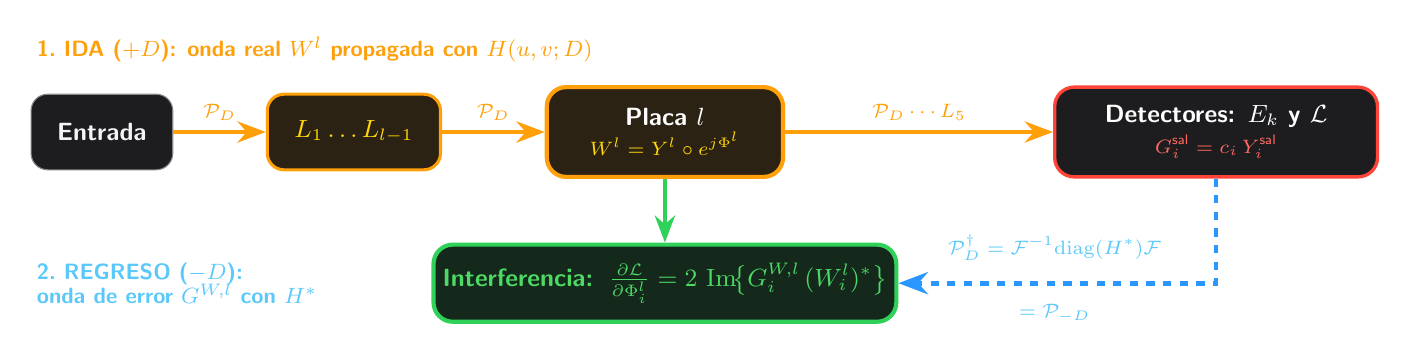
\begin{tikzpicture}[font=\sffamily,>=Stealth]

% Título arriba
\node[anchor=west,text=amber,font=\sffamily\bfseries\footnotesize] at (0,3.55)
  {1.\ IDA ($+D$): onda real $W^l$ propagada con $H(u,v;D)$};

% Nodos de propagación adelante
\node[draw=muted,fill=boxbg,rounded corners=6pt,minimum width=1.8cm,minimum height=0.96cm,text=lighttext,font=\sffamily\bfseries\small] (ent) at (0.95,2.50) {Entrada};

\node[draw=amber,fill=amberbg,line width=1.1pt,rounded corners=6pt,minimum width=2.2cm,minimum height=0.96cm,text=amberlight,font=\sffamily\bfseries\small] (prev) at (4.15,2.50) {$L_1 \dots L_{l-1}$};

\node[draw=amber,fill=amberbg,line width=1.5pt,rounded corners=7pt,minimum width=3.0cm,minimum height=1.14cm,text=white,align=center] (pl) at (8.10,2.50)
  {\textbf{\small Placa $l$}\\[-1pt]\scriptsize\color{amberlight}$W^l = Y^l \circ e^{j\Phi^l}$};

\node[draw=redaccent,fill=boxbg,line width=1.2pt,rounded corners=7pt,minimum width=4.1cm,minimum height=1.14cm,text=white,align=center] (det) at (15.10,2.50)
  {\textbf{\small Detectores: $E_k$ y $\mathcal{L}$}\\[-1pt]\scriptsize\color{redlight}$G^{\text{sal}}_i = c_i\,Y^{\text{sal}}_i$};

% Flechas adelante
\draw[->,amber,line width=1.6pt] (ent) -- node[above,font=\scriptsize\bfseries,text=amber]{$\mathcal{P}_D$} (prev);
\draw[->,amber,line width=1.6pt] (prev) -- node[above,font=\scriptsize\bfseries,text=amber]{$\mathcal{P}_D$} (pl);
\draw[->,amber,line width=1.6pt] (pl) -- node[above,font=\scriptsize\bfseries,text=amber]{$\mathcal{P}_D \cdots L_5$} (det);

% Título abajo a la izquierda (bien separado de la caja verde)
\node[anchor=west,text=cyanlight,font=\sffamily\bfseries\footnotesize,align=left] at (0,0.58)
  {2.\ REGRESO ($-D$):\\[-1pt]onda de error $G^{W,l}$ con $H^*$};

% Caja verde de interferencia holográfica
\node[draw=greenaccent,fill=greenbg,line width=1.5pt,rounded corners=7pt,minimum width=5.7cm,minimum height=0.98cm,text=greenlight,align=center] (grad) at (8.10,0.58)
  {\textbf{\small Interferencia:}\;\;\small$\frac{\partial\mathcal{L}}{\partial\Phi_i^l} = 2\,\operatorname{Im}\!\bigl\{G_i^{W,l}\,(W_i^l)^*\bigr\}$};

% Flecha vertical W^l -> interferencia
\draw[->,greenaccent,line width=1.5pt] (pl.south) -- (grad.north);

% Regreso (-D)
\draw[->,blueaccent,line width=1.7pt,dashed] (det.south) |- (grad.east);
\node[anchor=south,text=cyanlight,font=\sffamily\scriptsize\bfseries] at (13.05,0.74)
  {$\mathcal{P}_D^\dagger = \mathcal{F}^{-1}\mathrm{diag}(H^*)\mathcal{F}$};
\node[anchor=north,text=cyanlight,font=\sffamily\scriptsize\bfseries] at (13.05,0.44)
  {$= \mathcal{P}_{-D}$};

\end{tikzpicture}
\end{document}
